\section{Werkpakket 2: Prototyping}
2. Prototyping V0.1 (4 maanden) 

Het doel van het prototype is om zo snel mogelijk alle afzonderlijke stappen te testen en bewijzen dat het werkt. Het zal in een virtuele omgeving draaien waarbij makkelijk geïtereerd kan worden. Portabolt zal een interface ontwikkelen waarmee extern de batterijen aangestuurd kunnen worden. Er zal een communicatielaag worden gebouwd waarmee AIP de batterijen kan aansturen. Er wordt een testprotocol ontwikkeld waarmee elke afzonderlijke stap getest en gevalideerd kan worden. 
Deliverables: 
1. Portabolt sturingsinterface 
2. Koppeling tussen All in power, Portabolt, Edge, Envitron 
3. Werkend prototype in gesimuleerde omgeving 

Uren begroot: 1720

Opbouwen van de sandbox. We gaan eerst alles in dit prototype volledig digitaal ontwikkelen om te kijken of het werkt en waar we tegen aan lopen. Daarvoor gaan we een aantal modules ontwikkelen. Deze modules zijn de price generation module, de energy profile simulation en de optimization module. We gaan in deze fase nog geen daadwerkelijke data van het internet scrapen, maar alleen bewijzen dat alles werkt.   

\subsection{1. Price Generation Module}
\textbf{Objective:} Simuleer dynamische elektriciteitsprijzen die elke dag om 12:00 uur gegenereerd worden voor de volgende dag. \\
\textbf{Input:} Random variabelen die de prijzen beïnvloeden (bijv. vraag, aanbod, weersomstandigheden). \\
\textbf{Output:} Een array met 24 prijzen, één voor elk uur van de volgende dag.

Deze genereert elke keer dat je de code runt een array met prijzen. Er is een trend in gehardcorde waarmee we een normaal dagelijkse prijsschommeling simuleren. 

\begin{figure}[h!]
  \centering
  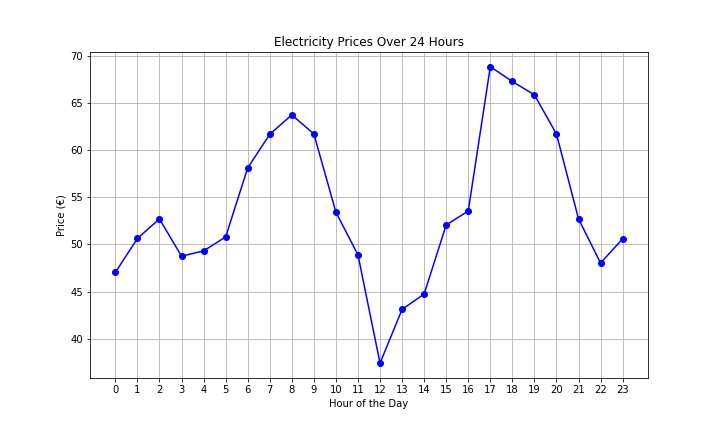
\includegraphics[width=\textwidth]{../docs/figures/price_generation_plot.png}
  \caption{Electricity Prices Over 24 Hours}
  \label{fig:price_plot}
\end{figure}

\FloatBarrier  % Voorkomt dat de afbeelding voorbij dit punt zweeft

\subsubsection{2. Energy Profile Simulation}

\textbf{Objective:} Creëer een energieverbruiksprofiel voor een gemiddeld bedrijf, dat per uur varieert. \\
\textbf{Input:} Kenmerken van het bedrijf (bijv. grootte, type industrie). \\
\textbf{Output:} Een array met 24 energieverbruikswaarden, één voor elk uur van de dag.

Hiermee simuleren we een willekeurig energieprofiel van een bedrijf. 

\subsection{Doel van de simulatie}
Het doel is om een representatief energieverbruikspatroon van een gemiddeld bedrijf te simuleren. Dit kan bijvoorbeeld per uur, dag, week of maand worden gegenereerd. Het profiel kan variëren afhankelijk van het type bedrijf, werkuren, seizoensinvloeden en andere factoren.

\subsection{Belangrijke variabelen}
\begin{itemize}
    \item \textbf{Bedrijfsprofiel:} Werkuren, industrietype, locatie, enz.
    \item \textbf{Baseload:} Het minimum energieverbruik van het bedrijf gedurende een dag (bv. verlichting, servers).
    \item \textbf{Piekbelasting:} Het maximale energieverbruik tijdens piekuren.
    \item \textbf{Dagelijks variërend verbruik:} Gebaseerd op het type bedrijf en de werkuren.
    \item \textbf{Seizoensgebonden variatie:} Verwarmings- of koelbehoeften.
    \item \textbf{Weekends en feestdagen:} Mogelijk lager verbruik.
\end{itemize}

\subsection{Simulatiemethoden}
\begin{itemize}
    \item \textbf{Random generation:} Gebruik een stochastisch model om het energieverbruik te genereren met een bepaalde spreiding rond gemiddelde waarden.
    \item \textbf{Tijdreeksanalyse:} Op basis van historische data (indien beschikbaar) kun je een tijdreekspatroon simuleren.
\end{itemize}

\subsection{Python Code Structuur}
De code kan worden gestructureerd met de volgende componenten:

\subsubsection{Main Simulation Script (main.py)}
Dit bestand start de simulatie, genereert het energieprofiel, en visualiseert het resultaat.
\begin{itemize}
    \item Initialiseer de simulatie.
    \item Roep de functies aan om energieverbruiksprofielen te genereren.
    \item Plot de resultaten.
\end{itemize}

\subsubsection{Company Profile (company\_profile.py)}
Dit script bevat functies om een bedrijfsprofiel te definiëren (bv. industrieel, kantoor, winkel). Elke categorie kan specifieke energiebehoeften en patronen hebben.

\begin{verbatim}
def define_company_profile():
    # Return een standaard bedrijfsprofiel op basis van categorie.
\end{verbatim}

\subsubsection{Energy Profile Generator (energy\_profile.py)}
Bevat de logica om het energieverbruiksprofiel te genereren.

\begin{verbatim}
def generate_daily_profile(company_profile):
    # Genereert het dagelijkse energieverbruik op basis van bedrijfsprofiel.
    
def apply_seasonal_variation(profile):
    # Past seizoensgebonden variaties toe op het energieprofiel.

def simulate_weekends(profile):
    # Voegt weekend- en feestdagvariaties toe.
\end{verbatim}

\subsubsection{Utilities (utils.py)}
Handige functies voor bijvoorbeeld het genereren van random verbruikswaarden, plotten van de data, etc.

\subsection{Simulatieverloop}
\begin{itemize}
    \item Genereer eerst een basis energieprofiel voor een gemiddelde dag.
    \item Pas vervolgens variaties toe voor piekbelasting, weekends, en seizoensgebonden schommelingen.
    \item Resultaten visualiseren met grafieken om een duidelijk overzicht van het verbruik te geven.
\end{itemize}

\subsection{GitHub-structuur}
Maak de volgende mappen en bestanden in de \texttt{energyprofile} folder:

\begin{verbatim}
energyprofile/
├── main.py
├── company_profile.py
├── energy_profile.py
├── utils.py
└── data/
    └── (eventuele historische data of configuratiebestanden)
\end{verbatim}

\subsection{Visualisatie}
Gebruik bijvoorbeeld \texttt{matplotlib} om het energieverbruik door de tijd te plotten.



\subsubsection{3. Optimization Module (Trading Algorithm)}
\textbf{Objective:} Beslis wanneer elektriciteit moet worden gekocht of verkocht, gebaseerd op prijsfluctuaties en het energieverbruik van het bedrijf. \\
\textbf{Input:} Prijsarray en energieverbruiksarray. \\
\textbf{Output:} Een optimalisatiestrategie die maximale winst oplevert door elektriciteit op het laagste punt te kopen en op het hoogste punt te verkopen.
